\documentclass{article}
\usepackage[utf8]{inputenc}
\renewcommand\thesection{\Alph{section}}
\usepackage[a4paper, margin=1in]{geometry}
\usepackage{amssymb}
\usepackage{amsmath}
\usepackage{amsthm}
\usepackage[thinc]{esdiff}
\usepackage{graphicx}
\usepackage[dvipsnames]{xcolor}
\usepackage{mdframed}
\usepackage{hyperref}

\mdfdefinestyle{pstyle}{linecolor=blue, backgroundcolor=red!5, nobreak=true}
\mdfdefinestyle{hstyle}{linecolor=blue, backgroundcolor=yellow!10, nobreak=true}
\mdfdefinestyle{sstyle}{linecolor=blue, backgroundcolor=green!5, nobreak=true}

\usepackage[british]{babel}
\usepackage[showdow]{datetime2}
\DTMlangsetup[en-GB]{ord=raise,monthyearsep={,\space}}
\DTMsetdatestyle{en-GB}

\newcommand{\ans}{\textbf{\emph{Answer}:}\: }


\newcounter{problem}[section]
\newenvironment{problem}[2][\today]{\refstepcounter{problem}\subsection{#1} \par\medskip
\begin{mdframed}[style=pstyle]
\textbf{Problem~\textit{\theproblem}. (\texttt{#2})}\\[1ex] }{\end{mdframed}\medskip}

\newcounter{hint}[subsection]
\newenvironment{hint}[1][]{\refstepcounter{hint} \par \medskip \begin{mdframed}[style=hstyle]
\textbf{Hint~\sffamily{\thehint}: \:}}
{ \end{mdframed} \medskip}

\newenvironment{solution}[1][]{\par \medskip \begin{mdframed}[style=sstyle] 
#1 \textbf{\emph{Solution}}. \\[1ex] } {\hfill \qedsymbol \\ \end{mdframed} \medskip}

\title{Problem of the week}
\author{Chirag Falor}
\begin{document}

\maketitle
\tableofcontents
\newpage
\section*{Introduction}

A compilation of all the Problems of the Week and their solutions until \today. Enjoy :) \textit{P}

\setcounter{section}{15}

\section{Physics}

\DTMsavedate{P1}{2021-01-10}
\begin{problem}[\DTMusedate{P1}]{MITx 8.02}
This one is an easy one, but a special one. Consider a circular plate charged capacitor of radius $r$ with charge $Q_0$. Fill it with a resistive liquid which conducts current $I(t)$ which is uniformly distributed in it. The distance between the plates is $d$, and $d \ll r$ to avoid end effects. Now consider a concentric loop inside the capacitor parallel to the plates of capacitor whose radius $a$, such that $a<r$. Find $\oint \vec{B} \cdot \vec{dl}$ around the loop at $t>0$.\\
\newline
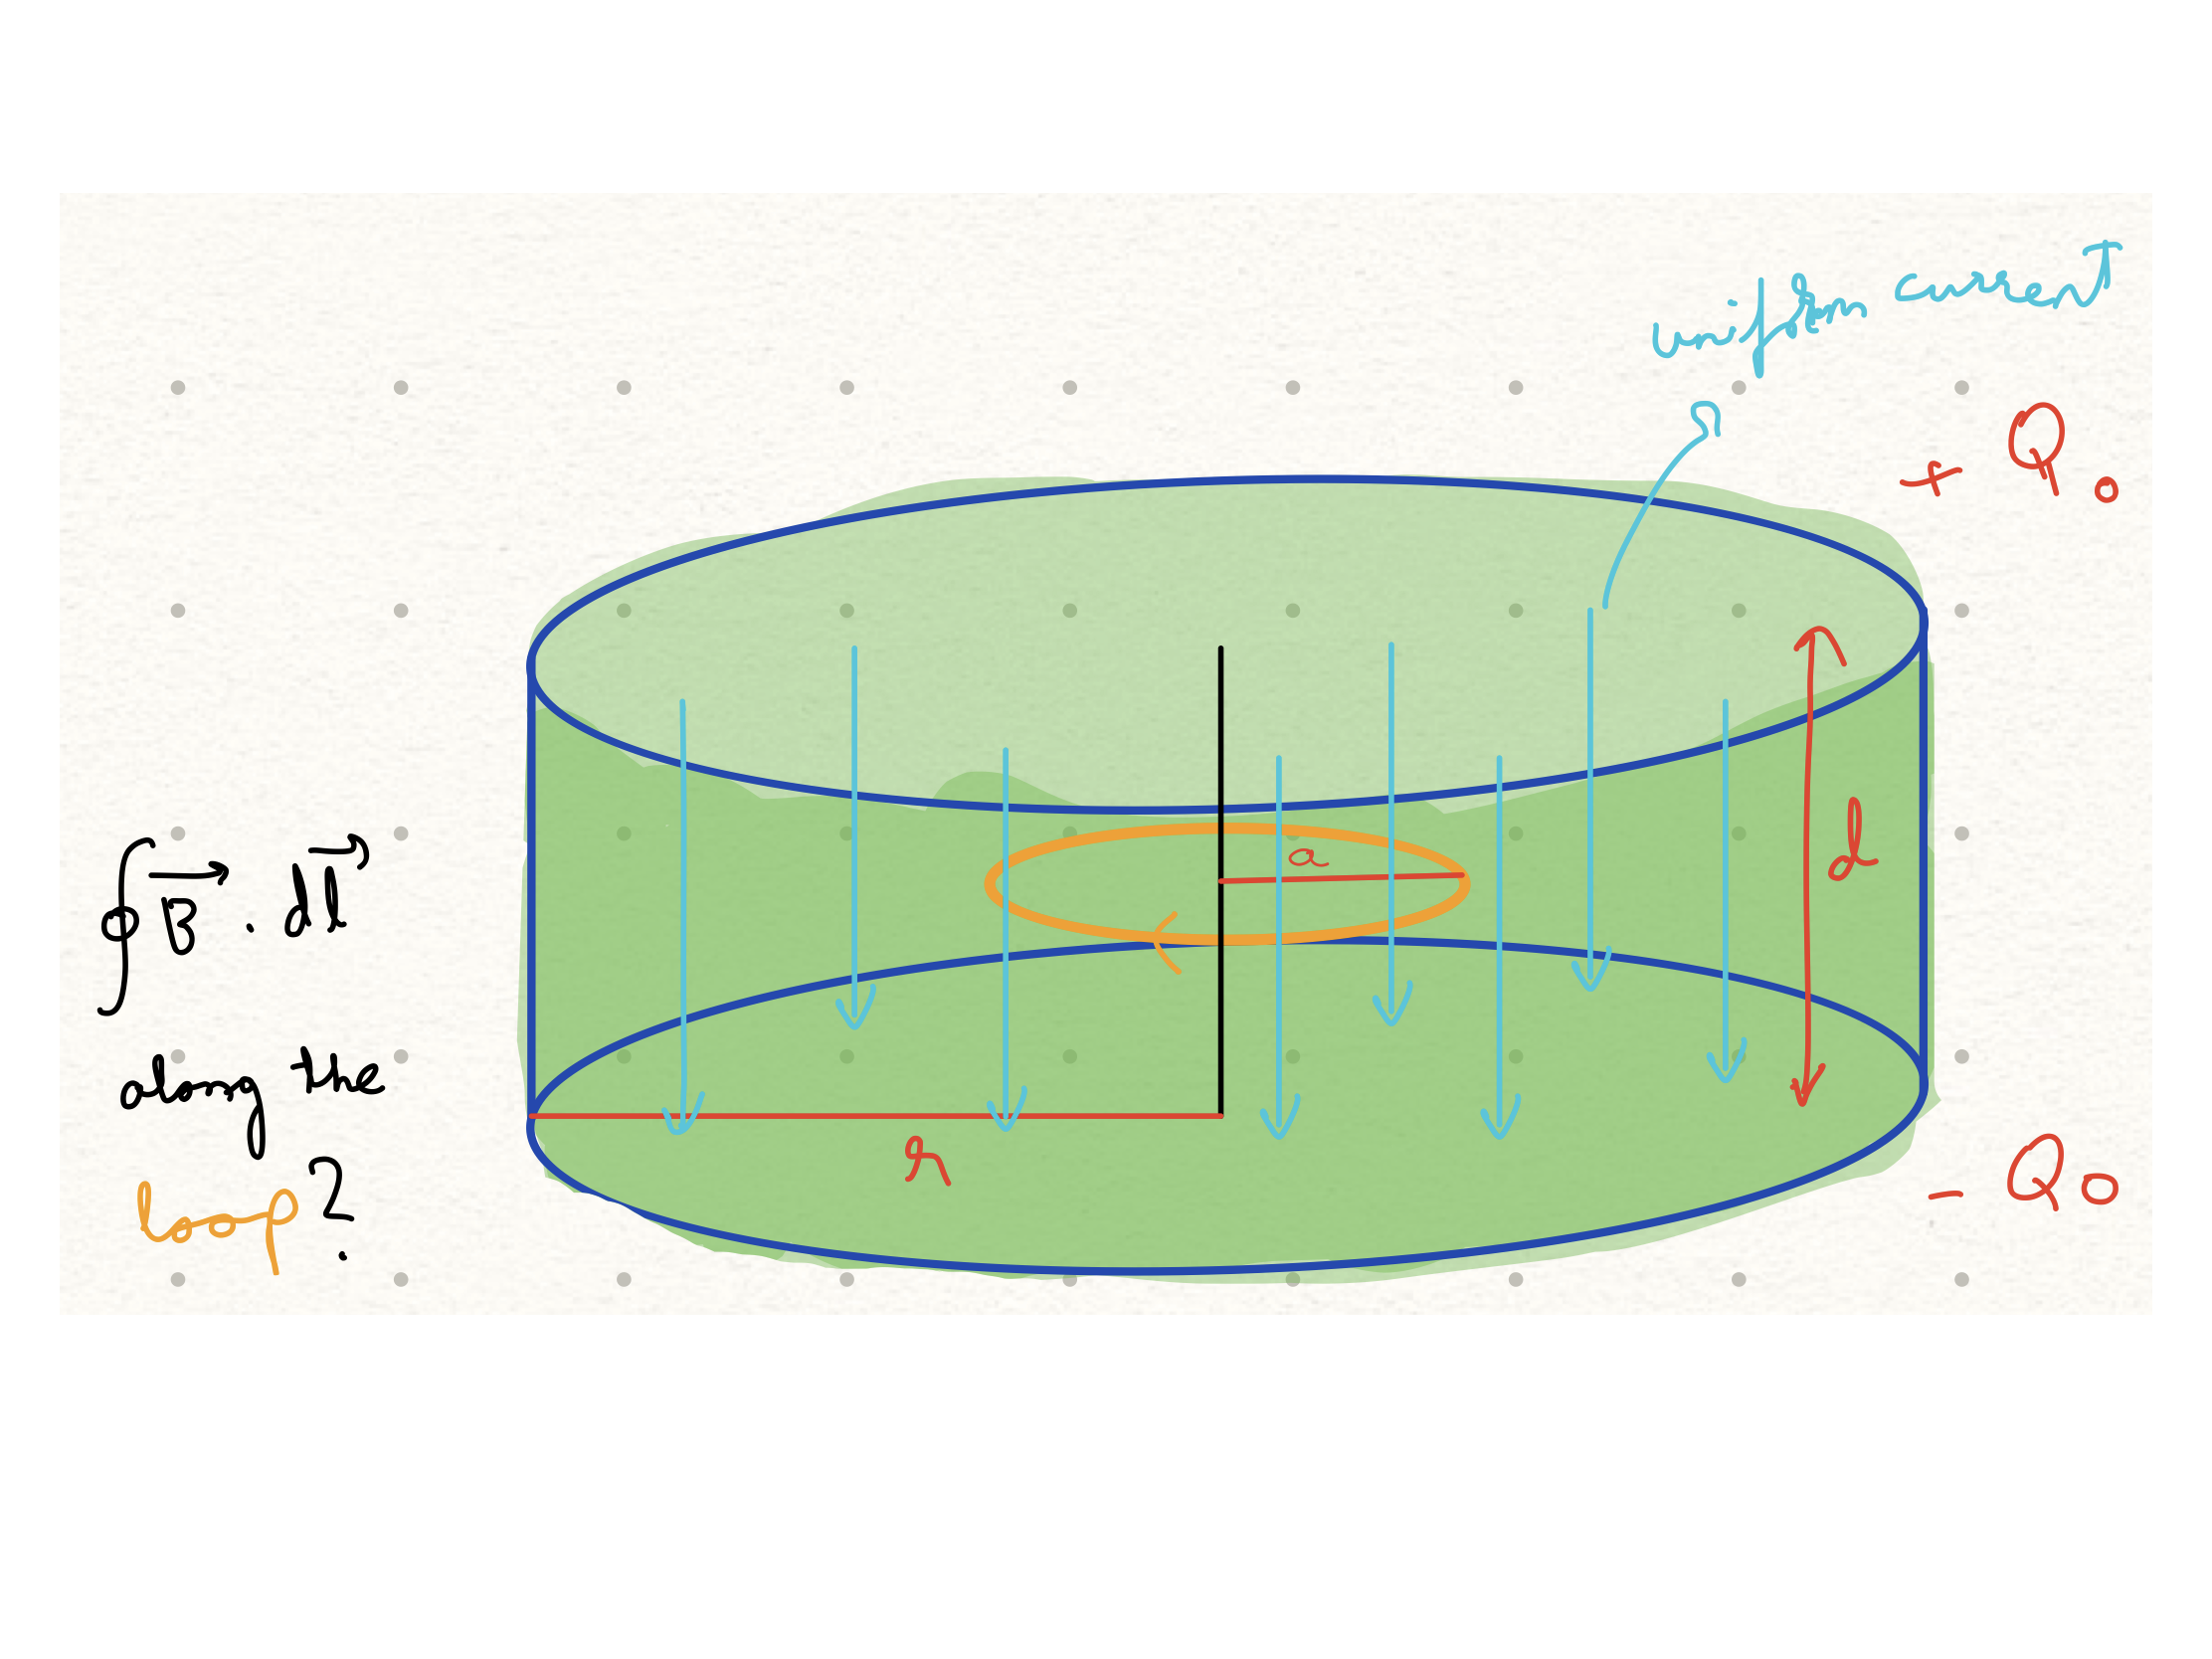
\includegraphics[width=\textwidth]{ProblemPictures/capacitor_resistiveliquid.PNG}
\end{problem}

% \begin{solution}
% Note: Electric field flux passing from the loop is $$\phi_E=\dfrac{\dfrac{Q_0}{\pi r^2}}{\epsilon_0} \times \pi a^2 = \dfrac{Q_0 a^2}{\epsilon_0 r^2}$$
% Current passing through loop is
% $$I_{current}= -\diff{Q_0}{t} \dfrac{a^2}{r^2}$$
% as the current in the loop is proportional to its area and negative sign as $Q_0$ is decreasing.\\
% By Ampere's law,

% \begin{align*}
%     \oint \vec{B} \cdot \vec{dl} &= \mu_0 \left( I_{current} +\epsilon_0 \diffp{\phi_E}{t} \right)\\
%     &= \mu_0\left(-\diff{Q_0}{t} \dfrac{a^2}{r^2} + \epsilon_0 \diffp{\left(\dfrac{Q_0 a^2}{\epsilon_0 r^2}\right)}{t}\right)\\
%     &= 0
% \end{align*}
% \ans $0$
% \end{solution}

% \DTMsavedate{P2}{2021-01-31}
% \begin{problem}[\DTMusedate{P2}]{Practice question given in class}
% The SHM of a ball with a cavity
% \end{problem}

% \DTMsavedate{P3}{2021-02-10}
% \begin{problem}[\DTMusedate{P3}]{original}
% Brachistrone problem
% \end{problem}



% \DTMsavedate{P4}{2021-02-10}
% \begin{problem}[\DTMusedate{P4}]{inspired while studying 18.02}
% curl and conservative forces
% \end{problem}

% \DTMsavedate{P5}{2021-02-10}
% \begin{problem}[\DTMusedate{P5}]{Inspired from recitation in 8.223}
% Wrapped string around cylinder, from recitation 3 8.223
% \end{problem}

















% \setcounter{section}{12}
% \section{Mathematics}

% \DTMsavedate{M1}{2021-01-17}
% \begin{problem}[\DTMusedate{M1}]{Inspired from JEE-Advanced 2020 P1 Maths Q.18}
% Many people didn't know how Taylor polynomials are useful and I am shocked. Firstly, and obviously, they are immensely useful in calculating limits. I would highly recommend to learn all the common Taylor series (if you haven't have till now) \url{https://en.wikipedia.org/wiki/Taylor_series#List_of_Maclaurin_series_of_some_common_functions}. Then solve this question (the best I could come up with for now). Find the Taylor series for $(1+x)^{\frac 1 x}$ (near $x=0$) till $3$ terms and use it to find
% \[\lim_{x \to 0} \dfrac{(1+x)^{-\frac 1 x} - \dfrac{1}{e}\left(1+\dfrac x 2 \right)}{x^2} \]
% \end{problem}

% \begin{solution}
% Differentiation of $(1+x)^{\frac{1}{x}}$ is not easy, so using $\log$ seems better.
% \begin{align*}
%     (1+x)^{\frac{1}{x}}&= e^{\dfrac{ \ln (1+x)}{x}}
%                         = e^{\dfrac{x - \dfrac {x^2}{2} + \dfrac {x^3}{3} + \cdots}{x}}
%                         = e^{1 - \dfrac x 2 + \dfrac {x^2}{3} + \cdots }\\
%                         &= e \left(1+ \left(- \dfrac x 2 + \dfrac {x^2}{3} + \cdots\right) +\dfrac{\left(- \dfrac x 2 + \dfrac {x^2}{3} + \cdots\right)^2}{2} +\cdots\right)\\
%                         &= e\left( 1 - \dfrac{x}{2} +\dfrac{x^2}{3} \cdots + \dfrac{x^2}{8} - \dfrac{x^3}{6} + \cdots \right)\\
%                         &= e\left(1-\dfrac{x}{2} +\dfrac{11 x^2}{24} +\cdots \right)
% \end{align*}
% Remember the above 3 terms; I have seen many questions using it. Now using it to find Taylor series of $(1+x)^{-\frac 1 x}$
% \begin{align*}
% (1+x)^{-\frac 1 x}&=\dfrac{1}{(1+x)^{\frac 1 x}}
%                 = \dfrac{1}{e\left(1 - \dfrac x 2 +\dfrac{11 x^2}{24} +\cdots \right)}\\
%                 &= \dfrac{1}{e}\left(1 - \left(- \dfrac x 2 +\dfrac{11 x^2}{24} +\cdots\right) + \left(-\dfrac{x}{2} +\dfrac{11 x^2}{24} +\cdots\right)^2 +\cdots \right)\\
%                 &= \dfrac{1}{e}\left(1 + \dfrac{x}{2} - \dfrac{11x^2}{24} \cdots + \dfrac{x^2}{4} + \cdots \right)\\
%                 &= \dfrac{1}{e}\left(1 + \dfrac{x}{2} - \dfrac{5x^2}{24} \cdots \right)
% \end{align*}
% Hence,
% \[\lim_{x \to 0} \dfrac{(1+x)^{-\frac 1 x} - \dfrac{1}{e}\left(1+\dfrac x 2 \right)}{x^2}=\lim_{x \to 0} \dfrac{\dfrac{1}{e}\left(1 + \dfrac{x}{2} - \dfrac{5x^2}{24} \cdots \right)- \dfrac{1}{e}\left(1+\dfrac x 2 \right)}{x^2}=-\dfrac{5}{24}\]
% \ans $-\dfrac{5}{24}$
% \end{solution}

% \DTMsavedate{M2}{2021-01-24}
% \begin{problem}[\DTMusedate{M2}]{Original}
% I came across/thought of this while browsing wikipedia page for definite improper integrals. It is a famous one, but don't try searching it without trying with the hints first. The problem is find
% \begin{equation}\label{DirichletInt}
%     \int_0^\infty \dfrac{\sin x}{x} \,  dx
% \end{equation}
% Note: This is actually difficult and took me an hour even when the concepts used to solve were fresh in my mind(albeit without any hint). The faint of the heart can wait for a hint.
% \end{problem}
% \begin{hint}
% Try finding this integral for any general $\alpha$
% \[\int_0^\infty e^{-\alpha x} \dfrac{\sin x}{x}\, dx\]
% \end{hint}

% \begin{hint}
% Try to use \href{https://en.wikipedia.org/wiki/Leibniz_integral_rule}{differentiation under integral sign}. (A tool through which \href{https://en.wikipedia.org/wiki/Leibniz_integral_rule#In_popular_culture}{Feynman got great reputation} for doing integrals)
% \end{hint}
% \begin{solution}
% Let
% \[f(\alpha)= \int_0^\infty e^{-\alpha x} \dfrac{\sin x}{x}\, dx\]
% Hence,
% \begin{align*}
%     f'(\alpha)&=-\int_0^\infty x e^{-\alpha x} \dfrac{\sin x}{x}\, dx
%         = -\int_0^\infty e^{-\alpha x} \sin x \, dx\\
%         &= \left(-\dfrac{e^{-\alpha x}}{\alpha^2+1} (-\alpha \sin x - \cos x)\right)\Big|_0^\infty\\
%         &=-\dfrac{1}{\alpha^2+1}
% \end{align*}
% Now,
% \begin{align*}
% f(\alpha)-f(0)&=\int_0^\alpha f'(t) \, dt = \int_0^\alpha f'(t) \, dt=\int_0^\alpha \dfrac{-1}{t^2+1} \, dt\\
% &= -\tan^{-1} t\Big|_0^\alpha = -\tan^{-1} \alpha
% \end{align*}
% Let $\alpha \to \infty$. We know that $\displaystyle{\lim_{\alpha \to \infty} f(\alpha) = 0}$, so
% \[ 0- f(0) = - \dfrac{\pi}{2}\\
% f(0)=\dfrac{\pi}{2}\\
% \int_0^\infty \dfrac{\sin x}{x} \,  dx\]
% \ans $\dfrac{\pi}{2}$\\
% Note: This integral is known as the \href{https://en.wikipedia.org/wiki/Dirichlet_integral}{Dirichlet integral}.
% \end{solution}
\end{document}
